The multi-model concept was introduced in \mf using GWF Model Exchange objects to support a tight coupling between any two groundwater flow models at the matrix level. This concept has proven to be successful and valued by the modeling community, but the implementation has had its drawbacks too. The information on the spatial discretization at the interface as it is available in the Model Exchange object is limited, designed to carry out the basic conductance calculation between connected cells but not sufficient for more advanced discretization schemes. For example, the XT3D option in the NPF package enables simulation of fully three-dimensional (3D) anisotropy by taking into account the full, three-dimensional conductivity tensor \cite{modflow6xt3d}. In doing so it requires geometrical data, not only from any pair of cells between which a flow needs to be calculated, but also from their neighboring cells. These data are not available in the Model Exchange object and the XT3D option could not be applied across the model interface, at least not without a significant restructuring of the code.

The extension of \mf with the transport model (GWT) comes with the need for a more generic coupling of sub-models too. Here the XT3D option is used in a similar fashion for the dispersion calculation, and the TVD (total variation diminishing) scheme in the advective transport calculation has a computational stencil that requires information from neighboring cells as well. Finally, the GWF Model Exchange object merely replicates logic already present in the standard GWF packages, e.g. the standard NPF conductance calculation, the Newton-Raphson formulation, or the cell rewetting algorithm, and is not easily adapted when additions or modifications to those packages are made. To address these challenges and extend \mf with the capability to couple GWT models, a more generalized method of coupling Numerical Models (currently GWF and GWT) has been developed.

The generalized coupling uses the concept of an Interface Model and is described in more detail below. In essence, this Interface Model uses the object-oriented paradigm in \mf to mimic a regular GWF or GWT model by means of type extension. This way it can use the existing packages and their algorithms in those models to calculate the coefficients for the matrix and right-hand-side vector in the Numerical Solution. Its grid is constructed around the interface defined by the Model Exchange with a sufficiently large extent to perform the calculations. Note that the Interface Model is never being solved and neither its configuration data nor its solution vector have any independent meaning: they are merely an image of those parts of the actual Numerical Models that contribute to the interface grid. As a matter of fact, and this is probably the most important point to make here, this generalized coupling with the Interface Model does not introduce any new model functionality. It even avoids the need for the alternative formulations currently present in the GWF Model Exchange. However, it does enable the user to apply the well-tested concepts of existing \mf packages not only on a model’s interior domain, but also across the interface between connected models.
  
\subsection{The Interface Model}
The generalized coupling is based on the Interface Model to provide the coefficients for the linear system in Numerical Solution. In order to utilize the routines in the existing flow and transport packages to calculate these coefficients, the grid for the Interface Model is constructed from the individual model grids and the coupling information specified by the user and its package data is kept synchronized with the model data during each step of the simulation. Because the Model Exchange makes it possible to connect model grids of different type (DIS, DISV, and DISU), the resulting interface grid is always unstructured, i.e. of type DISU.

Connecting models such that the dynamics at the interface can be described properly by an Interface Model does impose a few conditions on the configuration. For more advanced functionality such as XT3D, it is required that the relative position of the model grids is specified. They should also share the cell faces over which they are connected, such that the resulting grid for the interface can be specified as a valid DISU discretization. Another consequence is that a certain compatibility is required with respect to the active processes and configuration in the individual models: enabling advection (ADV) or dispersion (DSP), for example, only in one of two connected models introduces ambiguity in how to construct the Interface Model for the transport process. Similar arguments hold when two groundwater models are connected and only one of them is configured with a buoyancy package (BUY). Such model setups are currently not supported.

\begin{figure}[!t]
	\begin{center}
	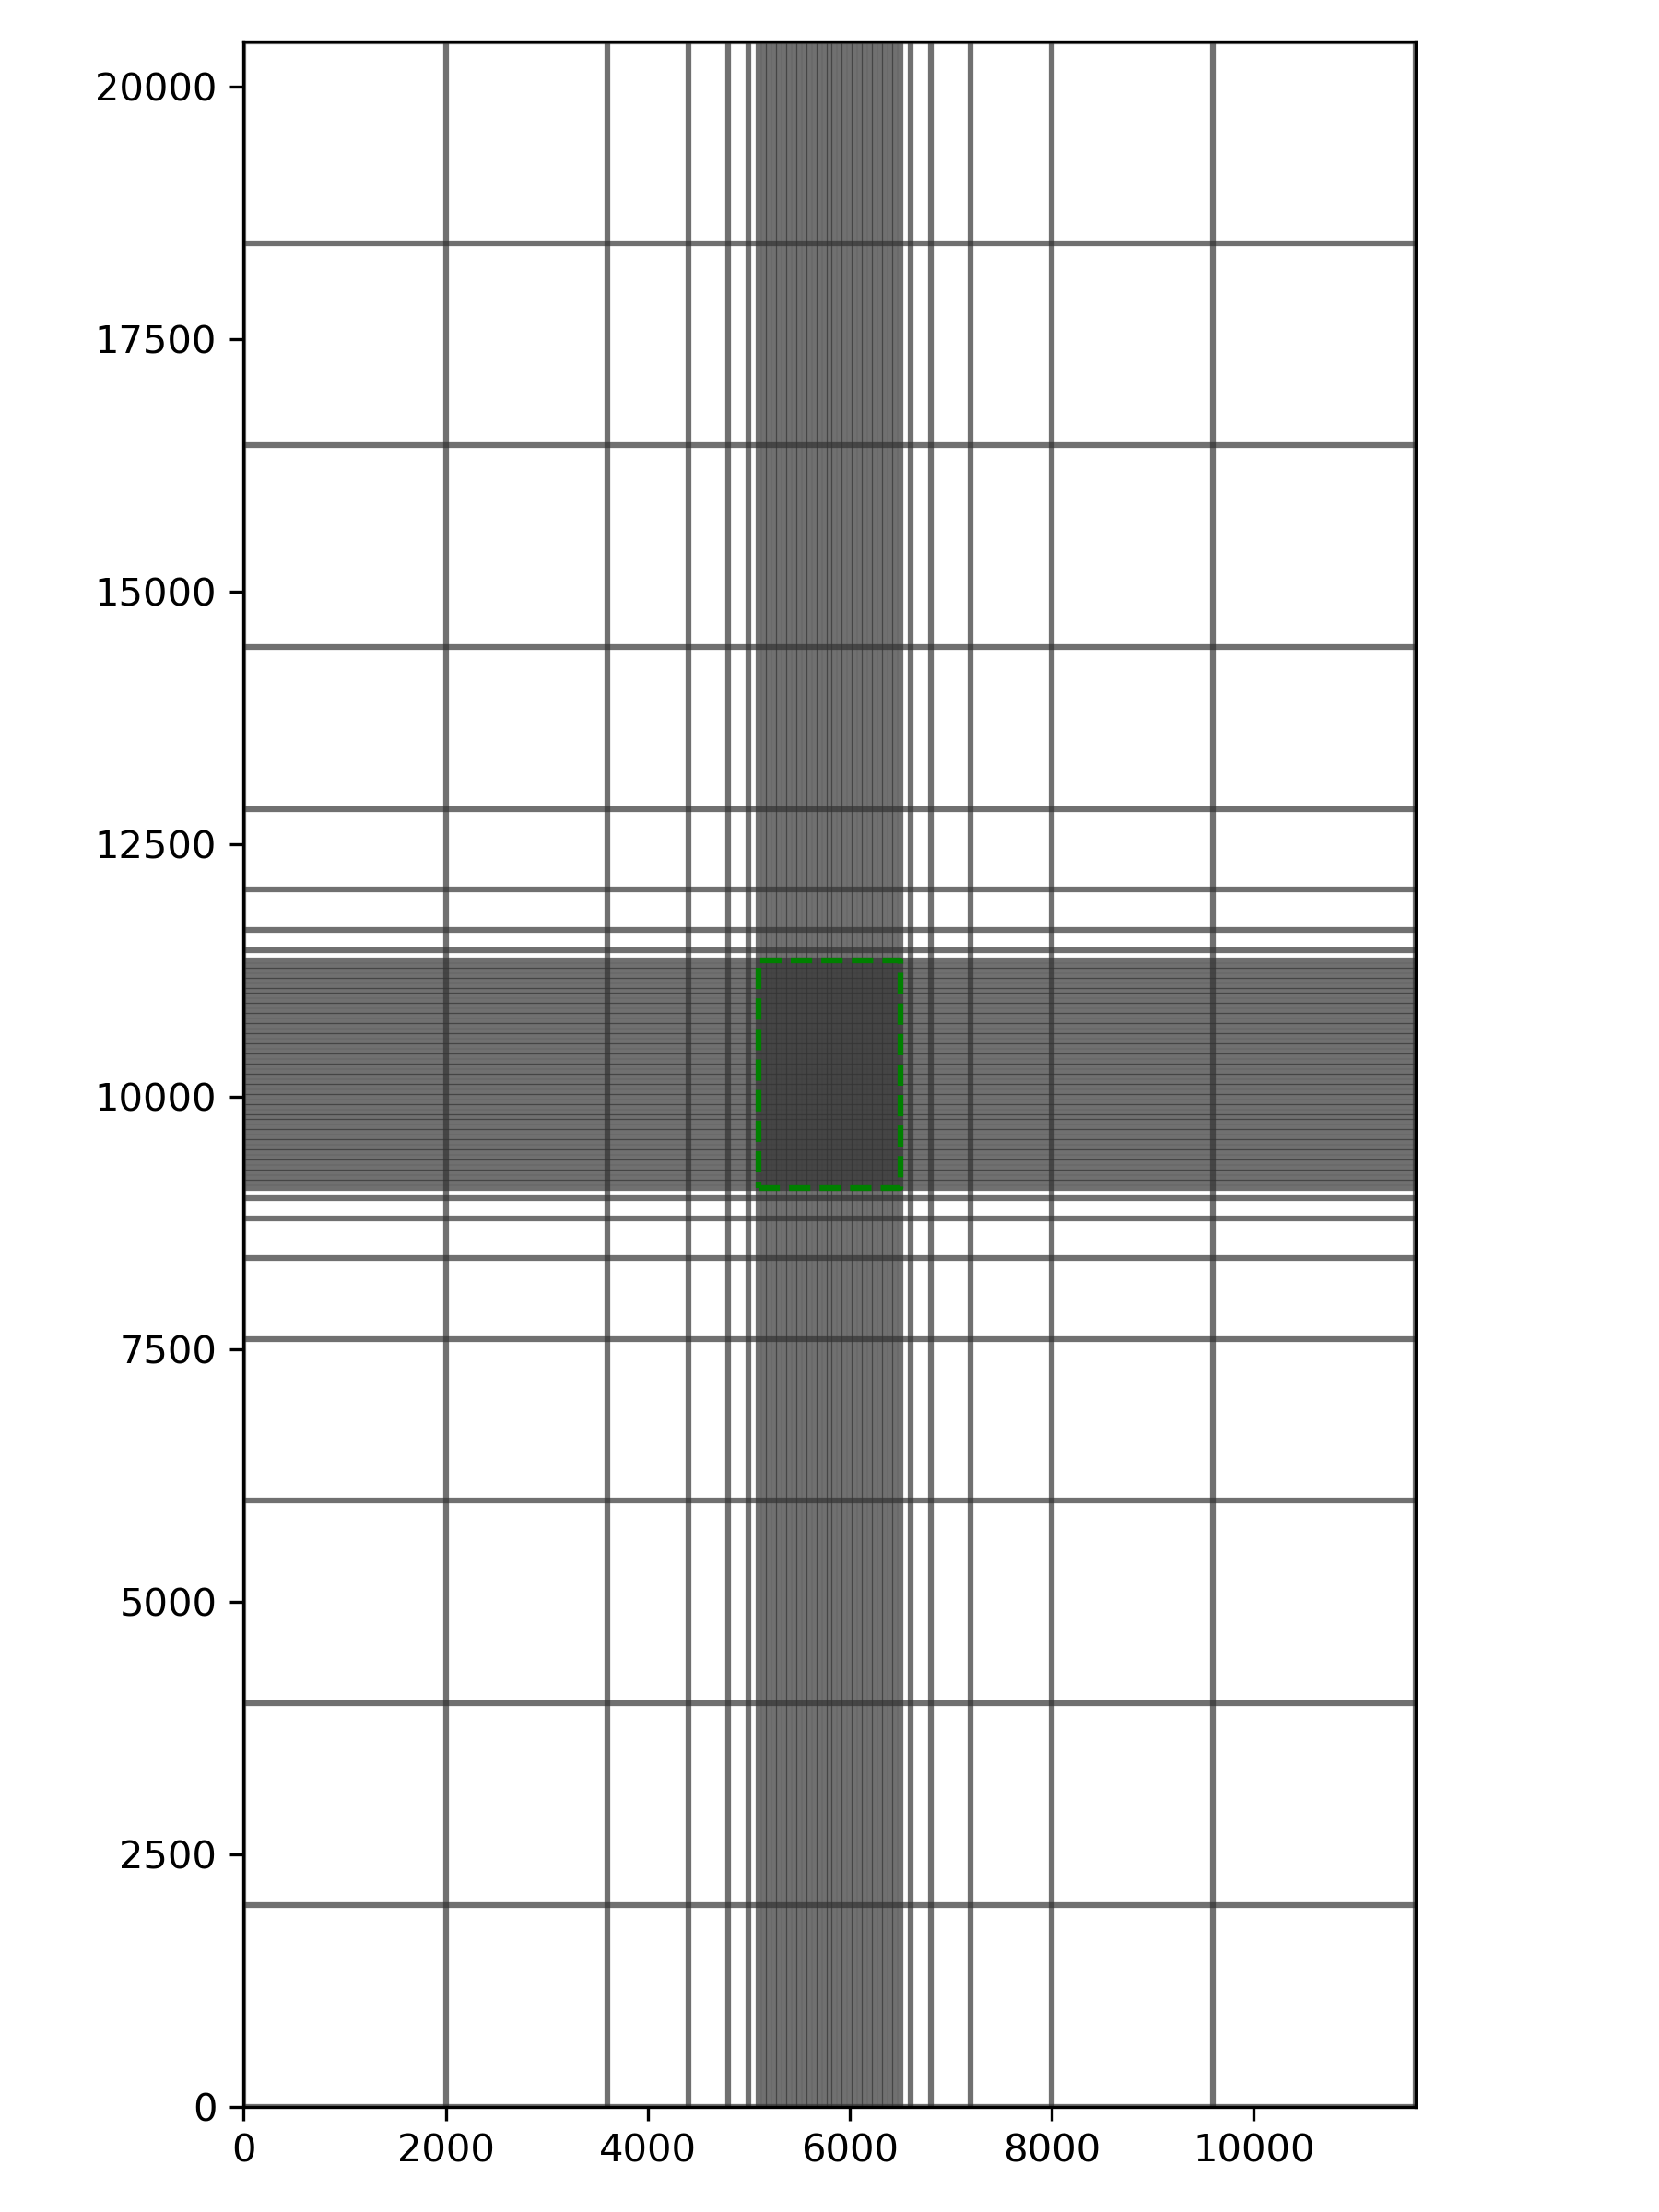
\includegraphics[width=0.5\textwidth]{./Figures/InterfaceModel/mt3dms-p10-modelgrid.png}
	\caption[A plan view of the model grid from MT3DMS problem 10]{A plan view of the model grid for the simulation as defined in MT3DMS problem 10. The red dashed rectangle shows the location of the interface that is used for decomposing this case into a system of coupled GWF and GWT models.}
	\label{fig:gwtgwt-fullgrid}
	\end{center}
\end{figure}

To illustrate the concept of this new coupling, a well known, single-model case study (problem 10 in the MT3DMS manual \cite{zheng1999mt3dms}) is implemented as a coupled system where the connection between the GWT models is handled by the Interface Model framework. This study is part of the official set of examples that comes with every \mf software release. The coefficients for the flow coupling in this case are calculated with the basic GWF Model Exchange module and the following discussion will focus on the GWT-GWT exchange. Figure~\ref{fig:gwtgwt-fullgrid} shows a plan view of the grid and the location of the interface between the submodels. Note that changing only the composition of the grid and leaving the model configuration the same, does not affect the outcome of the simulation\footnote{At the highest level of detail, the outcome does change because the numbering of the grid nodes is different in both scenarios leading to an equivalent but reordered matrix system to be solved. As expexted, these differences turn out to be well within the configured (IMS) solver tolerance.} and therefore makes for a very suitable test case of this coupling.

\begin{figure}[!ht]
	\begin{center}
	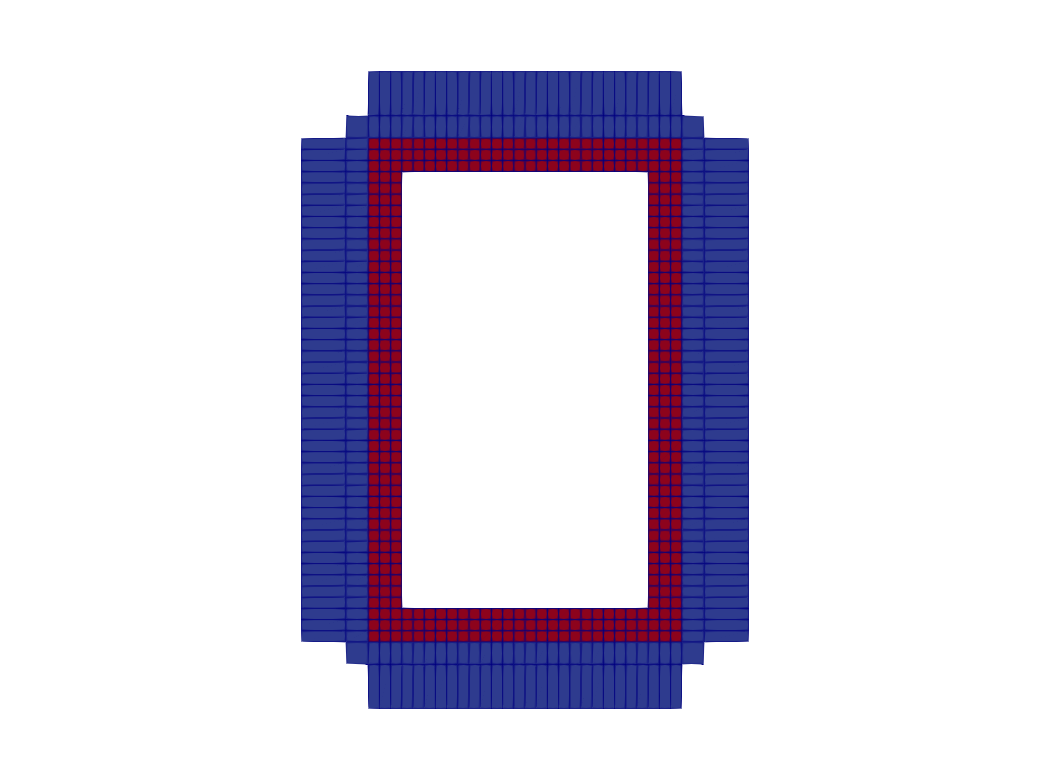
\includegraphics[width=0.8\textwidth]{./Figures/InterfaceModel/gwt-ifmod-grid.png}
	\caption[A top view of the Interface Model grid]{A top view of the grid for the Interface Model belonging to the inner GWT model in the example described in the text. The blue cells are located in the outer model’s grid, the red cells are internal. Note that deeper layers have an identical horizontal structure.}
	\label{fig:gwtgwt-interface-grid}
	\end{center}
\end{figure}

Figure~\ref{fig:gwtgwt-interface-grid} shows a plan view of the grid that is reconstructed as part of the Interface Model for the inner GWT model. The red band with cells belong to the inner model’s grid and the blue cells are part of the outer, coarser grid. Because two Interface Models are constructed for every Exchange, (one for each of the models in it) a similar though not identical picture can be drawn for the outer GWT model. However, the extent (or depth) of this grid is not necessarily equal on both sides of the exchange. The task of the Interface Model is twofold: First of all, it is designed to calculate the coefficients for the linear system for fluxes through the faces directly at the interface. Additionally, it can amend coefficients calculated by the submodel for those fluxes that would be affected by cells across the interface in case the simulation would have been set up as a single model. It is the requirement to support the latter that causes the asymmetry. This becomes clearer when looking at Figure~\ref{fig:gwtgwt-stencils} which shows the XT3D computational stencils (i.e. the group of cells required to compute the XT3D matrix coefficients for a flux through a particular cell face) and how they determine what the required extent of the interface grid is. To determine the flux through a face at the model interface, the cells on either side and their immediate neighbors are sufficient. To correctly calculate the flux through cell faces not directly at the interface but influenced by the connection to another model, more additional levels of connectivity are required, depending on the exact size of the computation stencil.

\begin{figure}[!ht]
	\begin{center}
	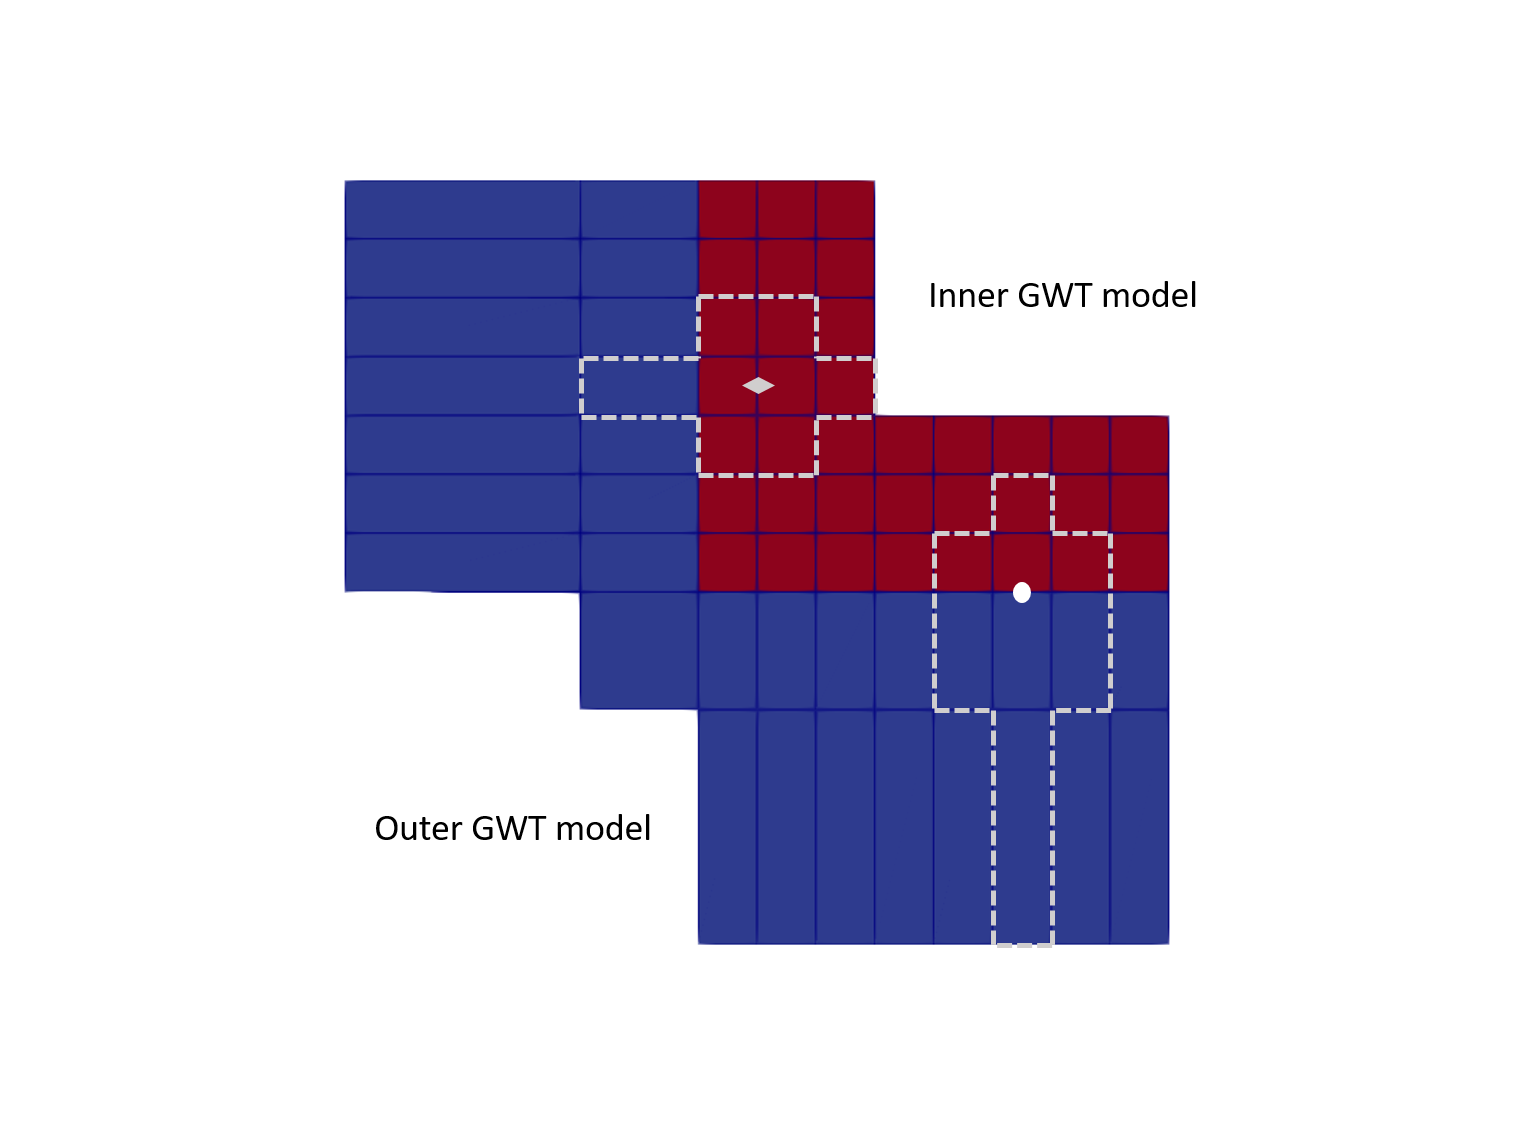
\includegraphics[width=0.8\textwidth]{./Figures/InterfaceModel/gwt-ifmod-stencils.png}
	\caption[Stencil size and the extent of the Interface Model grid]{Top view when zoomed in to the South-West corner of the interface grid. The dashed line surrounds the grid cells participating in the calculation of the dispersive XT3D flux directly at the interface (the white circle) and through a face in the model’s interior (the white diamond) which is nonetheless affected by the connection to the outer GWT model. The extension of the computational stencil in the vertical direction is omitted but straightforward.}
	\label{fig:gwtgwt-stencils}
	\end{center}
\end{figure}

This case study is used to demonstrate the concept of the generalized coupling method with the Interface Model. It serves as an excellent test case because the outcome should be identical to the known results, at least within the configured tolerance of the Numerical Solution. However, from a modeling perspective it would make more sense to redesign the model grid of the problem. With the new capability to use the multi-model approach also for problems containing solute transport, there is no longer a need to refine the study area by using varying column and row width as was done in the original MT3DMS problem. The outer grid can now be configured with a fixed cell shape without the unnecessary refinements, and the study area as a Local Grid Refinement (LGR), potentially even further refining its granularity without the need to set up the entire problem based on an unstructured DISU grid. 

Finally, such a LGR setup would allow to apply the Interface Model in another powerful way. A refinement of the grid is known to produce inaccuracies at the interface, as was already discussed in \cite{modflow6xt3d}. This can be remedied by enabling the XT3D option in the GWF NPF package. The new coupling mechanism based on the Interface Model makes it now possible to enable this option \emph{only} at the interface, which will mitigate the distorting effects of such a grid refiniment on the calculated flow field and still avoids the computational overhead of calculating the XT3D terms on the entire domain.

